\documentclass{article}

\usepackage{minted}
\usepackage[most]{tcolorbox}
\usepackage{geometry}
\usepackage{enumitem}
\usepackage{hyperref}
\usepackage{hyperref}
\usepackage[parfill]{parskip}
\usepackage{wrapfig}
\usepackage{accsupp}

\geometry{margin=0.8in}
\definecolor{lightgreen}{rgb}{0.56, 0.93, 0.56}
\definecolor{moonstoneblue}{rgb}{0.45, 0.66, 0.76}
\definecolor{magenta}{rgb}{0.8,0.66,0.76}
\begin{document}
\begin{flushright}
Computational Biology ~\\
Tufts University Bio 35 ~\\
Fall 2021 ~\\ ~\\
\end{flushright}
\begin{center}{\textbf{\Large{Spotlight 9: Scott Edwards}}}\end{center}

\textit{Please note that in general I have taken/adapted the words of our Spotlight subjects from their own websites to describe their work. I have done this in an effort to maintain accuracy in describing their research programs. Please do not copy paste text from their papers/websites in your assignments!}

\begin{wrapfigure}{L}{0.14\textwidth}
\begin{center}
 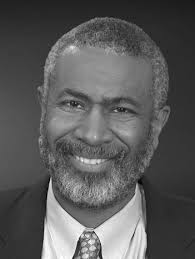
\includegraphics[width=0.13\textwidth]{images/scott-edwards.jpeg}
 \end{center}
\end{wrapfigure}
~\\ As part of our unit on biogeography and speciation, we are going to explore the work of Scott Edwards. Many of the research questions studied by Prof. Edwards' lab are motivated by natural history observations. Genomics and studies of genome evolution provide a remarkable window into the molecular basis of interesting phenotypic variation. Prof. Edwards has had a long-term interest in seabirds of the order \textit{Procellariformes}, which includes the albatrosses and petrels. These birds, with their long-distance foraging journey and remarkable life histories, are not only inspiring but also offer a treasure-trove of interesting molecular ecology facts to discover. Dr. Edwards is a Professor at Harvard University.
~\\

Please read the following article, on which Prof. Edwards is a co-author: 
\begin{enumerate}
\item \texttt{\href{https://www.eurekalert.org/pub_releases/2019-04/hu-ftk041719.php}{https://www.eurekalert.org/pub\_releases/2019-04/hu-ftk041719.php}}
\end{enumerate}

Also listen to the following podcast:
\begin{enumerate}
\item \texttt{\href{https://www.rnz.co.nz/national/programmes/saturday/audio/201764787/scott-edwards-birds-and-dinosaurs}{https://www.rnz.co.nz/national/programmes/saturday/audio/201764787/scott-edwards...}}
\end{enumerate}

Optionally, you may also be interested in this short piece on Prof Edwards:
\begin{enumerate}
\item \texttt{\href{https://news.harvard.edu/gazette/story/2020/07/harvard-ornithology-professor-bicycles-across-the-us/}{https://news.harvard.edu/gazette/story/2020/07/harvard-ornithology-professor...}}
\end{enumerate}


\subsubsection*{Written Assignment} 
After reading Scott Edwards' article and listening to the podcast, write a reflection (max one page) on what you discovered. You might wish to address some of the following: 

\begin{enumerate}
\item What was most interesting to you in reviewing these resources?
\item What did you learn from these resources about convergent evolution? How do computational tools and/or genomic data open up new avenues for exploration in convergent evolution studies?
\item What new questions do you have after reviewing these resources?
\item What do these resources tell you about the types of people that do computational biology research, or their motivations?
\end{enumerate}
\EndAccSupp{}


\end{document}